\newpage
\section{A lineáris programozás alapfeladata, kétváltozós grafikus megoldás és Fourier-Motzkin elimináció}

Egy egyenlőtlenségrendszer megoldásai közül kiválasztani azt, amely valamilyen
célfüggvény szerint optimális:

\begin{displaymath}
max(cx: Ax \leq b).
\end{displaymath}

Az elemek méretei: 

\begin{displaymath}
\begin{bmatrix} 1 &  \cdots &  n \end{bmatrix}
\begin{bmatrix} 1 \\ \vdots \\  n \end{bmatrix}
:
\begin{bmatrix} 1 & \cdots & n \\ \vdots & \ddots & \vdots \\ m  & \cdots & 0 \end{bmatrix}
\begin{bmatrix} 1 \\ \vdots \\  n \end{bmatrix}
\leq
\begin{bmatrix} 1 \\ \vdots \\  m \end{bmatrix}.
\end{displaymath}

Ha az egyenletnek, vagy a feladat más alakban van megadva átalakítható az
következő összefűggések alapján:
\begin{align*}
\alpha x \geq \beta  \Rightarrow  &-\alpha x \leq -\beta \\
\alpha x  =    \beta \Rightarrow  & -\alpha x \leq-\beta \\
									 & +\alpha x \leq+\beta \\
min(cx:Ax \leq b)	 \Rightarrow    & max((-c)x:Ax \leq b)
\end{align*}

A minimumos egyenlet megoldása a maximum egyenlet megoldásának az ellentétje lesz.
A kérdések, amelyre választ keressünk:
\begin{itemize}
  \item Létezik e $Ax \leq b$ egyenletnek megoldása?
  \item $cx$ korlátos e a megoldás halmazon?
  \item Melyik $x$--re maximális a $cx$ kifejezés?
\end{itemize}

\subsection{Kétváltozós feladat grafikus megoldása}

$\alpha x \leq \beta$ egyenlet meghatároz egy fél sikot, amelyet $\alpha x = \beta$
határol. Ha a félsíkok metszete véges, egy konvex sokszöget alkotnak, amely megadja a
megoldás halmazt.

\begin{figure}[htbp]
\centering
\subfigure{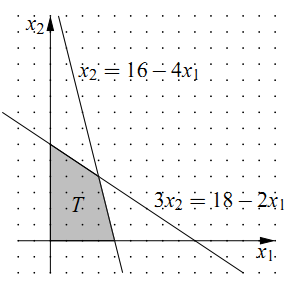
\includegraphics[height=6cm]{./kepek/2valtozo_megoldas_rajz.png}
\quad 
\subfigure{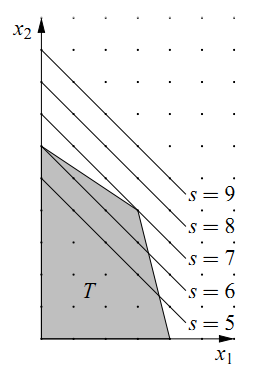
\includegraphics[height=6cm]{./kepek/2valtozo_megoldas_terulet.png} }}
\caption{Kétváltozós feladat grafikus megoldása} \label{fig:KetValtGraf}
\end{figure}

Ha a célfüggvényt különböző $x$--re felrajzoljuk meghatározható az optimális megoldás és az
ehhez tartozó $x$ értékek.

\subsection{Fourier-Motzkin elimináció}

Ennek segítségével megvizsgálhatjuk az egyenlet megoldhatóságát: $n$ változós egyenletet
visszavezetjük $n-1$ változóra, iteratívan, amíg egyváltozós egyenletrendszert nem kapunk;
erre könnyű megoldhatóságot vizsgálni. A folyamat:

\begin{enumerate}
  \item Minden egyenlet $\alpha \in \mathbb{R}^+$ szorzással az alábbi alakra hozható:
  \begin{displaymath}
  \begin{bmatrix}
  1  & A_+ \\
  -1 & A_- \\
  0  & A_0
  \end{bmatrix}
  \begin{bmatrix}
  x_1 & 
  x'
  \end{bmatrix}
  \leq
  \begin{bmatrix}
  b_+ \\
  b_- \\
  b_0
  \end{bmatrix}.
  \end{displaymath}
  \item 
  \begin{itemize}
  	\item Ha $A_-$ üres ($=\emptyset$): 
  	\begin{align*}
  	1 \cdot x_1 + A_+ x'     &\leq b_+ \\
  	1 \cdot x_1 + \alpha x' &\leq \beta \\
  	x_1 			  &\leq \beta - \alpha x' 
  	\end{align*} 
    Ekkor válasszuk úgy $x_1$--t, olyan kicsire hogy az összes sora e feltétel
    teljesüljön. Ezután $A_+$ teljes sorai elhagyható, továbbá elég $A_0$
    sorait vizsgálni, elhagyva a baloldalon található nulla oszlopot ($n-1$
    változós eset).
  	
  	\item Ha $A_+$ üres ($=\emptyset$): 
  	\begin{align*}
  	-1 \cdot x_1 + \alpha x'     &\leq \beta \\
  	x_1 			  &\geq \alpha x' - \beta 
  	\end{align*} 
  	Ekkor válasszuk úgy $x_1$--t, olyan nagyra hogy e feltétel teljesüljön.
  	Ezután $A_-$ elhagyható.
  	\item Ha $A_- \neq \emptyset$ és $A_+ \neq \emptyset$ akkor legyen 
  	$i \in A_-$ egy sora, $j \in A_+$ egy sora, és képezzük az összes sora az
  	alábbi ősszeget (ez exponenciális egyenletszaporodást jelent, e miatt az algoritmus
  	futási ideje is exponenciális):
  	\[
  	\left( \alpha_i + \alpha_j \right) \cdot x' \leq b_i + b_j 
  	\]
  	Ezzel visszavezettük a kérdést $n-1$ változós estre.
  \end{itemize}
 \item Ha $n=1$ és 
 \begin{align*}
 \exists~b_0 < 0 &\Rightarrow \mbox{nem megoldható} \\
 \not \exists~A_+ \mbox{ vagy} \not \exists~A_- < 0 &\Rightarrow \mbox{megoldható} \\
 \mbox{másképp igaz, hogy } x_1 \leq \beta_+ \mbox{ és } y_1 \geq \beta_-
 &\Rightarrow \mbox{megoldható ha } \mbox{max}(-\beta_-) \leq min(\beta_+)
 \end{align*} 
  Ha $n \geq 1$ folytassuk a $2$--es lépéstől.
\end{enumerate} 
